\section{The zero-level cobordism}\label{sec:obstruction}

We continue with the normalized family from Section~\ref{sec:morse}: its unique critical point is zero, its local model is the fixed $q_{k,l}$, its data at infinity are smooth and homogeneous, and~\eqref{eq:unbalanced-indices} holds. Put
\[
 Y=S^{k+l-1},\qquad
 \Sigma=\{q_{k,l}=0\}\cap Y\cong S^{k-1}\times S^{l-1}.
\]
Choose radii $a,R_0$ with collars in the local quadratic and outer homogeneous regions, respectively. Identify their annulus with $Y\times[0,1]$ by a smooth increasing radius $r(t)$, with $r'>0$. Write
\[
 s_b(u,t)=\frac{f_b(r(t)u)}{r(t)^2}.
\]
Near $t=0$ and $t=1$ this function is independent of $t$, and equals $q_{k,l}|_Y$ and the angular infinity data $h_b^1$, respectively. Differentials in this section are in the annulus variables, with $b$ fixed; we also write $f_b$ for its pullback to the annulus.

\subsection{A regular band and its two complementary regions}

Since $f_b$ has no critical point on the annulus and
\begin{equation}\label{eq:zero-level-differential}
 df_b=r^2ds_b\quad\text{on }s_b=0,
\end{equation}
zero is a regular value of $s_b$. Its zero set is transverse to both end faces. Compactness gives a small uniform $\epsilon>0$ and a band identification
\begin{equation}\label{eq:zero-band}
 C_b=\{s_b=0\},\qquad
 \mathcal R_b=\{\abs{s_b}\leq\epsilon\}\cong C_b\times J,
 \qquad J=[-\epsilon,\epsilon].
\end{equation}
To obtain it, choose a field with $ds_b$-derivative one in a slightly larger band, tangent to the end faces and purely angular and independent of $t$ on their collars. Such choices patch because the condition $ds_b(V)=1$ is affine. Integrating the field identifies its second coordinate with $s_b$. At the incoming end the choice can be fixed independently of $b$, so the resulting collar embedding $\Sigma\times J\hookrightarrow Y$ is fixed.

\begin{lemma}\label{lem:signed-flows}
On
\[
 P_{\pm,b}=\{(u,t):\ \pm s_b(u,t)\geq\epsilon\}
\]
there are smooth fields $V_{\pm,b}$, depending smoothly on $b$, such that
\begin{align}
 \pm df_b(V_{\pm,b})&>0 &&\text{on }P_{\pm,b},\label{eq:field-f}\\
 dt(V_{\pm,b})&>0 &&\text{near }t=0,1,\label{eq:field-t}\\
 \pm ds_b(V_{\pm,b})&>0 &&\text{on }s_b=\pm\epsilon.\label{eq:field-s}
\end{align}
The fields can be chosen with a common prescription extending across the whole angular sphere on each end collar.
\end{lemma}

\begin{proof}
By~\eqref{eq:zero-level-differential}, near the zero set a field can make $df_b$ and $ds_b$ both strictly positive, or both strictly negative. The same holds at the two side levels for small uniform $\epsilon$. On an end collar write $s_b=h$, angular and independent of $t$, and use
\[
 V=\partial_t+h\nabla_Yh.
\]
Then
\[
 dt(V)=1,\quad ds_b(V)=h\norm{\nabla_Yh}^2,\quad
 df_b(V)=h\bigl(2rr'+r^2\norm{\nabla_Yh}^2\bigr).
\]
These give the required signs, including strictness on the side levels, since $dh\ne0$ near $h=0$. Away from the prescribed regions, use strict signed gradient ascent or descent for $f_b$. Convex patching preserves every applicable strict linear inequality, and can keep the displayed prescription on smaller end collars. The construction is smooth over the compact parameter space. Fields on cornered regions are understood to extend locally across their faces.
\end{proof}

Let $T_-^0$ and $T_{-,b}^1$ be the truncated negative domains $s_b\leq-\epsilon$ on the inner and outer spheres, viewed in angular coordinates. They are isotopic to the respective negative tubes.

\begin{lemma}\label{lem:residual-hcob}
The negative field gives an embedding
\[
 j_b:T_-^0\hookrightarrow\Int T_{-,b}^1
\]
which is a homotopy equivalence. It also identifies $C_b$ with
\[
 T_{-,b}^1\setminus\Int j_b(T_-^0).
\]
In particular, the family $C_b$, with its fixed incoming identification with $\Sigma$, is a smooth family of h-cobordisms.
\end{lemma}

\begin{proof}
For $V_{-,b}$ the inner face and side face are entry faces, and the outer face is the only exit. Every trajectory exits in finite forward time: on the compact region $P_{-,b}$, $-df_b(V_{-,b})$ has a positive lower bound and $f_b$ has bounded range. Backwards, the same argument forces a trajectory to reach an entry face.

Flow to the first intersection with $t=1$ maps each entry face smoothly and injectively into $T_{-,b}^1$. Transversality to the exit face gives smooth dependence of the exit time, also at the side's outer edge where the time is zero. Extensions across the corner faces show that these maps have full rank up to the edges. Their images meet precisely along the shared inner edge and otherwise are disjoint, by uniqueness of flow; backwards flow gives their union as the entire outer tube. The image of the inner face lies in the interior of the outer tube, since the field points strictly inward from the side. The band identification~\eqref{eq:zero-band} identifies that side with $C_b$ and proves the stated decomposition.

Choose $\delta>0$ as in Lemma~\ref{lem:morse-sublevels}, also small enough that the sphere $a(S^{k-1}\times\{0\})$ in the fixed negative eigenspace lies in $f_b\leq-\delta$. This sphere is the core of the inner tube. Its image under the negative flow remains in this sublevel. The core represents a generator there by that lemma, and therefore its image at $R_0$ represents a generator in the outer radial portion. Angular projection carries it to a generator in the open negative domain. Inclusion of $T_{-,b}^1$ into this open domain is a homotopy equivalence for our small $\epsilon$. Thus $j_b$ has degree $\pm1$ on the sphere homotopy types of its source and target. These types are simply connected, so $j_b$ is a homotopy equivalence.

Excision with collars now gives
\[
 H_*(C_b,\partial_-C_b;\Z)
 \cong H_*(T_{-,b}^1,j_b(T_-^0);\Z)=0.
\]
This includes connectedness of $C_b$. The two tubes and their common boundary are simply connected, so van Kampen applied to the decomposition implies $\pi_1C_b=0$. The cobordism is orientable, and Poincar\'e--Lefschetz duality gives vanishing of the relative homology at its outgoing end as well. Both boundary components are diffeomorphic to $S^{k-1}\times S^{l-1}$ and hence simply connected. All these smooth spaces have CW type, so the homological Whitehead theorem \cite[Corollary~4.33]{Hatcher2002} makes both boundary inclusions homotopy equivalences. Regularity and properness give a smooth bundle of these cobordisms over $B$, including their boundary collars, with fixed incoming identification.
\end{proof}

\subsection{Stabilizing the cobordism inside a fixed cylinder}

The family $C_b$ gives a class $c_B\in[B,H(\Sigma)]$. We need a
product identification relative to the incoming end that varies over all
of $B$. We first thicken $C_b$ by one interval and
extend it to $Y$. The resulting family has a product complement in a
fixed cylinder. We will then use stability to recover the original
family class from this enlarged one.

In the space $H(X)$ recalled in Section~\ref{sec:tubes}, the incoming end is identified with $X$; when
$\partial X\ne\varnothing$, the vertical boundary is the prescribed
product $\partial X\times I$. There is no identification of the outgoing
end with $X$. All these data have collars. Equivalently one may bend the
vertical face into the outgoing face, so incoming and outgoing boundaries
meet along $\partial X$. This is the collared model of
\cite[Definitions~1.1.1 and~1.1.3]{WJR2013}. The product component is
\[
 H(X)_0\simeq BP(X),\qquad
 P(X)=\Diff(X\times I\ \mathrm{rel}\
 X\times\{0\}\cup\partial X\times I),
\]
with the equivalent convention of diffeomorphisms fixed near the indicated
faces and product near the outgoing face. Thus a null classifying map
into this component gives a product family relative to the incoming end.

In our application, $\Sigma$ is simply connected and has dimension at least $38$.
The smooth $h$-cobordism theorem
\cite[Theorem~9.1]{Milnor1965} makes every $h$-cobordism on $\Sigma$ a
product relative to its incoming end: its dimension is at least $39$,
and its boundary inclusions are homotopy equivalences. If a product
parametrization restricts to $a:\Sigma\to\Sigma$ at the incoming end,
precomposing it with $a^{-1}\times\id_I$ fixes that end pointwise.
Thus $H(\Sigma)$ is connected.

The interval stabilization used here is
$\sigma:H(X)\to H(X\times J)$, where $J$ is a closed interval. For $X$
closed and $C$ an $h$-cobordism from $X$ to $N$, add a fixed incoming
collar to form
\[
 C^-=(X\times[-1,0])\cup_X C.
\]
Use $C^-\times J$, with the following faces before rounding:
\begin{equation}\label{eq:stabilization-faces}
 \begin{aligned}
 \text{incoming: }&X\times\{-1\}\times J,\\
 \text{vertical: }&X\times[-1,0]\times\partial J,\\
 \text{outgoing: }&(N\times J)\cup(C\times\partial J).
 \end{aligned}
\end{equation}
The vertical face has its stated product identification; the remaining
sides belong to the outgoing end. Corner bending turns these into the
usual collared cobordism faces. For manifolds with boundary, retain the
existing product vertical faces as well and round their product corners.
This is the product construction of \cite[Definition~1.1.3]{WJR2013}.

If $e:X\hookrightarrow Y$ is a codimension-zero embedding, extension
$e_!:H(X)\to H(Y)$ glues the cobordism to the trivial cylinder on
$Y\setminus\Int e(X)$ along the product vertical boundary. In the bent
collared model, the same operation is
\begin{equation}\label{eq:hcob-extension}
 C\longmapsto(Y\times I)\cup_{X\times I}C,
\end{equation}
where $X\times I\subset C$ is the incoming collar. This expression shows
that extension commutes with interval stabilization, using the product
collars and their fixed corner adjustments.

Add trivial collars $Y\times[-1,0]$ and $Y\times[1,2]$ to the annulus and set, with corners to be rounded,
\begin{equation}\label{eq:band-cobordism}
 W_b=(Y\times[-1,0])\cup\mathcal R_b.
\end{equation}
Its incoming boundary is the fixed $Y\times\{-1\}$.
Figure~\ref{fig:regular-band} records these faces and the complementary
regions used below.
\begin{figure}[tbp]
\centering
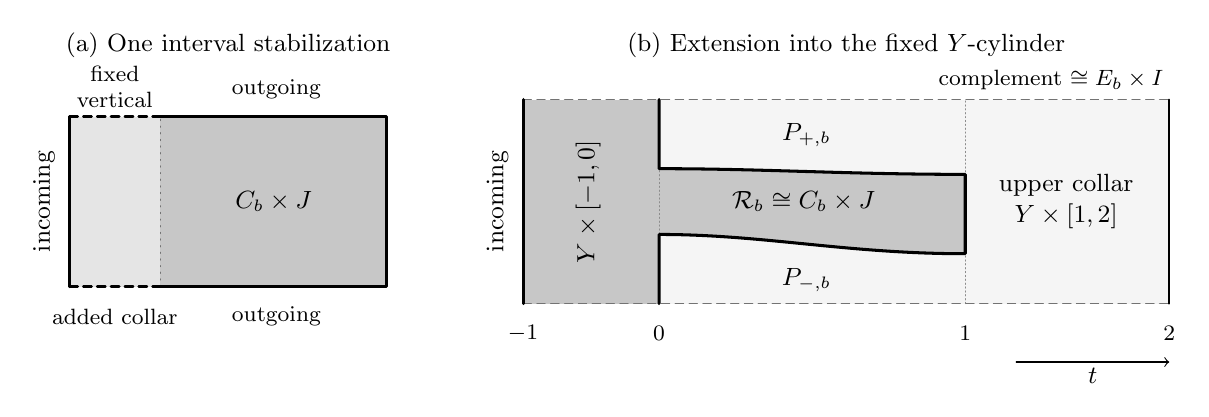
\begin{tikzpicture}[x=0.72cm,y=0.72cm,font=\small,
  every node/.style={inner sep=2pt},line cap=round,line join=round]
  \node at (2.8,5.25) {(a) One interval stabilization};
  \fill[black!10] (0,1) rectangle (1.6,4);
  \fill[black!22] (1.6,1) rectangle (5.6,4);
  \draw[line width=1.1pt] (0,1)--(0,4);
  \draw[densely dashed,line width=0.9pt] (0,1)--(1.6,1);
  \draw[densely dashed,line width=0.9pt] (0,4)--(1.6,4);
  \draw[black!55,dotted] (1.6,1)--(1.6,4);
  \draw[line width=1.1pt] (1.6,1)--(5.6,1)--(5.6,4)--(1.6,4);
  \node[rotate=90] at (-0.45,2.5) {incoming};
  \node at (3.6,2.5) {$C_b\times J$};
  \node[align=center,font=\footnotesize] at (0.8,4.53)
    {fixed\\vertical};
  \node[font=\footnotesize] at (3.65,4.48) {outgoing};
  \node[align=center,font=\footnotesize] at (0.8,0.47)
    {added collar};
  \node[font=\footnotesize] at (3.65,0.47) {outgoing};

  \node at (13.7,5.25) {(b) Extension into the fixed $Y$-cylinder};
  \fill[black!4] (8,0.7) rectangle (19.4,4.3);
  \fill[black!22] (8,0.7) rectangle (10.4,4.3);
  \path[fill=black!22]
    (10.4,1.92) .. controls (12.25,1.92) and (13.7,1.58) .. (15.8,1.58)
    --(15.8,2.98) .. controls (13.7,2.98) and (12.25,3.08) .. (10.4,3.08)
    --cycle;
  \draw[black!45,densely dotted] (10.4,0.7)--(10.4,4.3);
  \draw[black!45,densely dotted] (15.8,0.7)--(15.8,4.3);
  \draw[black!55,densely dashed] (8,0.7)--(19.4,0.7);
  \draw[black!55,densely dashed] (8,4.3)--(19.4,4.3);
  \draw[line width=1.1pt] (8,0.7)--(8,4.3);
  \draw[line width=0.7pt] (19.4,0.7)--(19.4,4.3);
  \draw[line width=1.1pt]
    (10.4,0.7)--(10.4,1.92)
    .. controls (12.25,1.92) and (13.7,1.58) .. (15.8,1.58)
    --(15.8,2.98)
    .. controls (13.7,2.98) and (12.25,3.08) .. (10.4,3.08)
    --(10.4,4.3);
  \node[rotate=90] at (7.55,2.5) {incoming};
  \node[rotate=90] at (9.15,2.5) {$Y\times[-1,0]$};
  \node at (12.95,2.5) {$\mathcal R_b\cong C_b\times J$};
  \node at (13.0,3.68) {$P_{+,b}$};
  \node at (13.0,1.12) {$P_{-,b}$};
  \node[align=center] at (17.58,2.5) {upper collar\\$Y\times[1,2]$};
  \node[anchor=east,font=\footnotesize] at (19.4,4.65)
    {complement $\cong E_b\times I$};
  \node[font=\footnotesize] at (10.4,0.18) {$0$};
  \node[font=\footnotesize] at (8,0.18) {$-1$};
  \node[font=\footnotesize] at (15.8,0.18) {$1$};
  \node[font=\footnotesize] at (19.4,0.18) {$2$};
  \draw[->,thin] (16.7,-0.33)--(19.4,-0.33)
    node[midway,below] {$t$};
\end{tikzpicture}
\caption{Face bookkeeping for one fiber, before corner rounding.
In (a), the dashed segments are the fixed vertical faces on the added
incoming collar $\Sigma\times[-1,0]\times J$; both sides beyond that
collar are movable outgoing faces. In (b), the dark region is
$W_b=(Y\times[-1,0])\cup\mathcal R_b$, and its heavy interface with
the light complement is $E_b=\partial_+W_b$. The product identification
of the complement is proved over the possibly varying bundle $E\to B$.
The angular direction is schematic: the upper and lower dashed display
edges are not boundary faces of the closed sphere $Y$. The drawing
asserts neither radial monotonicity nor a product trivialization of
$C\to B$.}
\label{fig:regular-band}
\end{figure}


\begin{lemma}\label{lem:band-is-stabilization}
The family $W_b$ represents the extension to $Y$ of the interval stabilization of $C_b$.
\end{lemma}

\begin{proof}
Adjoin a fixed incoming collar to $C_b$, obtaining
\[
 C_b^-=(\Sigma\times[-1,0])\cup C_b.
\]
Its interval stabilization is $C_b^-\times J$, with incoming $\Sigma\times J$. In the convention of~\eqref{eq:stabilization-faces}, the two faces $C_b\times\partial J$ and the outgoing end times $J$ form the movable boundary. The added incoming-collar portions supply the fixed vertical boundary when a boundary-relative model is used. Extending across $\Sigma\times J\hookrightarrow Y$ replaces that incoming collar by $Y\times[-1,0]$. The result is exactly~\eqref{eq:band-cobordism}, using~\eqref{eq:zero-band} for the attached piece.

This construction works on transition maps as well. Local product trivializations of $C_b$ fix its incoming collar and can be made product on outgoing collars, without fixing their outgoing end. Extend them by identity over the added collar and take their product with $\id_J$. A fixed bending of the two interval coordinates gives the usual boundary-relative stabilized cylinder. Near the lower gluing seam the transitions are identity; near the upper seam they preserve both interval coordinates and act only in the remaining boundary variable. Thus fixed planar corner adjustments descend through the transitions. Extending by identity over the complement in $Y$ gives the same family as~\eqref{eq:band-cobordism}. This is a single interval stabilization with both side faces movable.
\end{proof}

\begin{lemma}\label{lem:product-complement}
The complement of $W_b$ up to $Y\times\{2\}$ is, after compatible corner rounding, a product cylinder over the outgoing boundary of $W_b$, smoothly in $b$. Consequently $[W]=0$ in $[B,H(Y)]$.
\end{lemma}

\begin{proof}
Before rounding, the outgoing boundary of $W_b$ comprises the two sign domains at $t=0$, the two band sides, and the band end at $t=1$. Its complement is the union of $P_{-,b}$ and $P_{+,b}$ with the upper collar $Y\times[1,2]$. Use Lemma~\ref{lem:signed-flows} on the sign regions. On and above the upper end, its common angular prescription extends across the band and has $dt>0$. It can be continued to the top with that property. The resulting field points from every outgoing face of $W_b$ into the complement, and its only exit face is $t=2$.

We describe a rounding transverse to this field. At a lower corner put
\[
 v=t,\qquad w=\pm s_b-\epsilon;
\]
the complement is the quadrant $v,w\geq0$. At an upper corner put $v=t-1$ and use the same $w$; the complement is the union $v\geq0$ or $w\geq0$. At either corner the field has $dv(V)>0$ and $dw(V)>0$. Round the interface by a curve in the first quadrant at the bottom, and in the third quadrant at the top, smoothly joining the unchanged straight parts. Choose its conormal into the complement as a nonzero nonnegative combination of $dv,dw$. This makes the rounded interface transverse with the same orientation.

The product end coordinates allow fixed small planar roundings over all parameters. If the stabilized piece and its exterior are kept as separate pieces at the bottom seam, move their dividing wall in the small corner neighborhood so it reaches the rounded interface transversely. All transition maps there are identity. Each piece is then a fixed planar adjustment of its original collared model, so Lemma~\ref{lem:band-is-stabilization} still describes the rounded family.

Every forward trajectory reaches $t=2$ in finite time. In sufficiently small lower and upper collars, $dt(V)$ has a uniform positive lower bound; this bounds transit time there and prevents reentry across their inner thresholds in the wrong direction. In the remaining compact middle, a trajectory stays in one sign region and its signed $f_b$ increases at a rate bounded below, with bounded range. Its time there is therefore finite. It cannot exit across the entry boundary. The same argument backwards reaches the rounded outgoing boundary of $W_b$.

Transversality gives smooth hitting times in the initial point and in $b$. Rescaling these times gives a product diffeomorphism of the complementary cobordism relative to its entry, say $E_b=\partial_+W_b$. This proves a product identification over the entire possibly varying bundle $E\to B$; it does not merely assert that the individual fibers are products.

Finally, adding $E_b\times I$ to the outgoing end changes no incoming-relative h-cobordism bundle class. Extend the transverse field a small uniform distance into $W$ to obtain a collar $E\times[-\eta,0]$. A fixed increasing smooth diffeomorphism $[-\eta,1]\to[-\eta,0]$, equal to the identity near $-\eta$, compresses the added cylinder into this collar, and is identity on the rest of $W$. It is defined without choosing a trivialization of $E\to B$. The enlarged total is the literal product $B\times Y\times[-1,2]$, relative to its incoming boundary. Hence $[W]=0$.
\end{proof}

\subsection{Recovering the original cobordism family}

We have shown that the extension to $Y$ of one interval stabilization
of $C_b$ is a product family. We now show that this operation detects
its class over $B=S^9$.

The stable parametrized $h$-cobordism theorem
\eqref{eq:stable-hcob-theorem} is natural for this extension
\cite[Theorems~0.1 and~0.3]{WJR2013}.

The quantitative statements needed below are as follows. The single
stabilization $H(X)\to H(X\times J)$ is $r$-connected provided
\begin{equation}\label{eq:igusa-range}
 \dim X\geq\max(2r+8,3r+5).
\end{equation}
Every subsequent stage also satisfies this dimension bound, so the map
$H(X)\to\Hs(X)$ is $r$-connected as well. Moreover, an
$(r+1)$-connected map $X\to Y$ induces an $r$-connected map
$\Hs(X)\to\Hs(Y)$. For the first statement we use Igusa's stability
theorem \cite{Igusa1988} in the form of
\cite[Theorem~2.16]{CP2025}; the second is
\cite[Theorem~2.17]{CP2025}. Extension is the map of
\cite[Definition~2.15]{CP2025}. As specified in
\cite[Remark~2.13]{CP2025}, these statements use the WJR product
convention \eqref{eq:stabilization-faces}. Connectivity here means isomorphisms on
$\pi_i$ for $i<r$ and a surjection on $\pi_r$.

\begin{proposition}\label{prop:hcob-injectivity}
Let $k,l\geq20$, and put
\[
 Y=S^{k+l-1},\qquad
 \Sigma=\{q_{k,l}=0\}\cap Y\cong S^{k-1}\times S^{l-1}.
\]
For a closed collar embedding $e:\Sigma\times J\hookrightarrow Y$, the
composite
\begin{equation}\label{eq:hcob-injectivity-map}
 H(\Sigma)\xrightarrow{\sigma}H(\Sigma\times J)
 \xrightarrow{e_!}H(Y)\longrightarrow\Hs(Y)
\end{equation}
induces an isomorphism on $\pi_9$ in the product component. Consequently,
if a sphere family in $H(\Sigma)$ has null image under this composite,
the family is itself null.
\end{proposition}

\begin{proof}
Here $\dim\Sigma=k+l-2\geq38$, whereas the bound in
\eqref{eq:igusa-range} for $r=10$ is $35$. Hence
$H(\Sigma)\to\Hs(\Sigma)$ is $10$-connected. The composite
$H(\Sigma)\to H(\Sigma\times J)\to\Hs(\Sigma\times J)$ has the same
connectivity: its target is the tail of the defining stabilization
telescope. It therefore induces an isomorphism on $\pi_9$.

Set $d=\min(k,l)-1$. The source of $e$ is $(d-1)$-connected, and
$Y$ has vanishing homotopy groups in degrees at most $d$. Thus $e$ is
$d$-connected: it is an isomorphism below degree $d$ and a surjection in
degree $d$. The stable extension
$\Hs(\Sigma\times J)\to\Hs(Y)$ is consequently $(d-1)$-connected,
with $d-1\geq18$, and also induces an isomorphism on $\pi_9$.
Compatibility of extension and stabilization identifies the composite of
these two isomorphisms with \eqref{eq:hcob-injectivity-map}.

The space $H(\Sigma)$ is connected, as shown above.
For a connected target, free homotopy classes of maps from $S^9$ are
orbits of based classes under the fundamental group action. The orbit
of zero is just zero. Thus the same detection of nullity applies to
sphere families without a specified basepoint.
\end{proof}

By Proposition~\ref{prop:hcob-injectivity}, Lemmas~\ref{lem:band-is-stabilization} and~\ref{lem:product-complement} imply
\begin{equation}\label{eq:zero-cobordism-class}
 c_B=0\quad\text{in }[B,H(\Sigma)].
\end{equation}
The passage to free sphere classes is harmless: the fundamental-group action fixes zero. The classification of smooth families by this h-cobordism space now supplies incoming-relative product trivializations of the whole family $C_b$, not just of its individual fibers; see \cite[Proposition~2.11]{CP2025}.

\subsection{Removing the cobordism and straightening the cores}

\begin{proof}[Completion of the proof of Proposition~\ref{prop:one-critical}]
First replace the outer negative domains by their truncated domains $T_{-,b}^1$; moving a regular boundary through a sufficiently small angular collar is an isotopy. By Lemma~\ref{lem:residual-hcob} and~\eqref{eq:zero-cobordism-class}, each of these domains is $j_b(T_-^0)$ with a smoothly varying product collar attached. Shrink that collar: if its product coordinate is $[0,1]$, retain only $[0,s]$ and let $s$ decrease to zero. The outer boundaries vary through embeddings, including at $s=0$, where they equal $\partial j_b(T_-^0)$. Thus the family is homotopic as tube domains to $j_b(T_-^0)$.

Fix $T_-^0\cong S^{k-1}\times D^l$ and let
\[
 e_b:S^{k-1}\hookrightarrow Y,\qquad e_b(u)=j_b(u,0)
\]
be its cores. We may replace $j_b(T_-^0)$ by small round normal neighborhoods of $e_b$. Here is a precise version that removes framing choices. First shrink its disk factors to a uniformly small radius. In metric normal-bundle charts of the cores write
\[
 j_b(u,z)=\bigl(\psi_b(u,z),\xi_b(u,z)\bigr),\qquad
 \psi_b(u,0)=u,\quad \xi_b(u,0)=0.
\]
On this smaller domain use, for $0<t\leq1$, the embeddings
\begin{equation}\label{eq:normal-linearization}
 (u,z)\longmapsto
 \bigl(\psi_b(u,tz),\ t^{-1}\xi_b(u,tz)\bigr).
\end{equation}
These are compositions of the original embedding with dilation in the disk and normal directions. The estimates $\norm{\xi_b(u,tz)}\leq Ct\norm{z}$ keep them in the chosen chart. At $t=0$ the formula extends smoothly to $(u,D_z\xi_b(u,0)z)$. The normal derivative is an isomorphism, so the limit is also an embedding. Its fiber ellipsoids can be changed to round balls by interpolation of positive definite metrics, with the common disk radius chosen sufficiently small. At the level of domains this requires no fixed normal framing.

The core family is homotopic through embeddings to the fixed standard core. Indeed, as maps into $Y=S^{k+l-1}$, both it and the constant standard family are nullhomotopic because
\[
 \dim(B\times S^{k-1})=k+8<k+l-1.
\]
Choose a smooth homotopy, constant on collars of its two time endpoints. Its parameter dimension, including time, is ten. Relative fiberwise multijet transversality avoids double points since
\[
 10+2(k-1)<k+l-1.
\]
Vertical rank-defect strata have codimension at least $l+1>10+(k-1)$ and are avoided as well.
Here we use the parametric multijet theorem in the form of
\cite[Theorem~2.3.4 and Corollary~2.3.5(iii)]{BPT2025}, and explain
its compact-parameter relative application. Cover the compact parameter
manifold $B\times[0,1]$, away from smaller endpoint collars, by finitely
many coordinate charts. In each chart multiply the local perturbations
by a parameter cutoff supported away from the endpoint collars. Local
source cutoffs allow independent variations at distinct source points,
as required for the two-point jets. Apply transversality successively on
compact subsets covering these charts; sufficiently small subsequent
perturbations preserve avoidance already obtained on compact subsets.
The rank estimate first gives fiberwise immersions. Compactness and
$C^1$ openness then give a uniform neighborhood of the diagonal on
which distinct sufficiently close source points remain distinct.
Apply the two-point argument on the compact complement of this
neighborhood. The strict dimension bounds make each transverse
bad-stratum preimage empty. The endpoint families remain fixed, and
their embedding property persists on smaller endpoint collars by
$C^1$ openness. This proves that every member of the resulting homotopy
is an embedding. Uniformly small round normal neighborhoods follow this
family to a fixed tube.

All the resulting homotopies of domains give homotopies of tube data. Use boundary collars for local defining-function choices; the fibers of these choices are convex, so partitions of unity in parameters give global choices. Continuous families in the smooth topology suffice for the homotopy class; when smooth parameter dependence is needed, relative approximation preserves embeddings and regularity on compact parameter sets. We have proved nullity of the enlarged family in $T_{k,l}$. Adding the missing negative squares returns to the diagonal system and proves the proposition.
\end{proof}
